The paper that truly brought to light the issue of adversarial attacks was
\cite{szegedy2014intriguing}. In this paper, they provide an optimization-based approach to
generating what are known as ``adversarial examples''. To do this, they trained multiple models with
fully-connected neurons on the MNIST training dataset\cite{lecun}. One of the networks was  an
autoencoder. After performing this task, they generated adversarial examples for the sake of
comparing the performance of the non-attacked network to the attacked network. In order to do this,
they used L-BFGS\cite{lbfgs} (modified to keep any changes within the $L_{\infty}$ norm) to try to
minimize the loss function, but with the target class being an incorrect class. They also made sure
that the predicted class of the modified image is indeed the class they were hoping to achieve, and
the modifications did not cause resulting input values to be less than zero or greater than one (the
bounds on the possible values in the image). This resulted in images (derived from the training set)
that visually still should not be misclassified, yet the neural network (and a few linear
regression-based models) misclassified them. In fact, they were able to get accuracy down to 0\%
using noise that one would not think could change the classifer's output. These kinds of corrupted
images were shown in their work, and are reproduced in Figure \ref{adversarialexamplespictures}.

\begin{figure}
    \begin{center}
        \begin{tabular}{c c}
            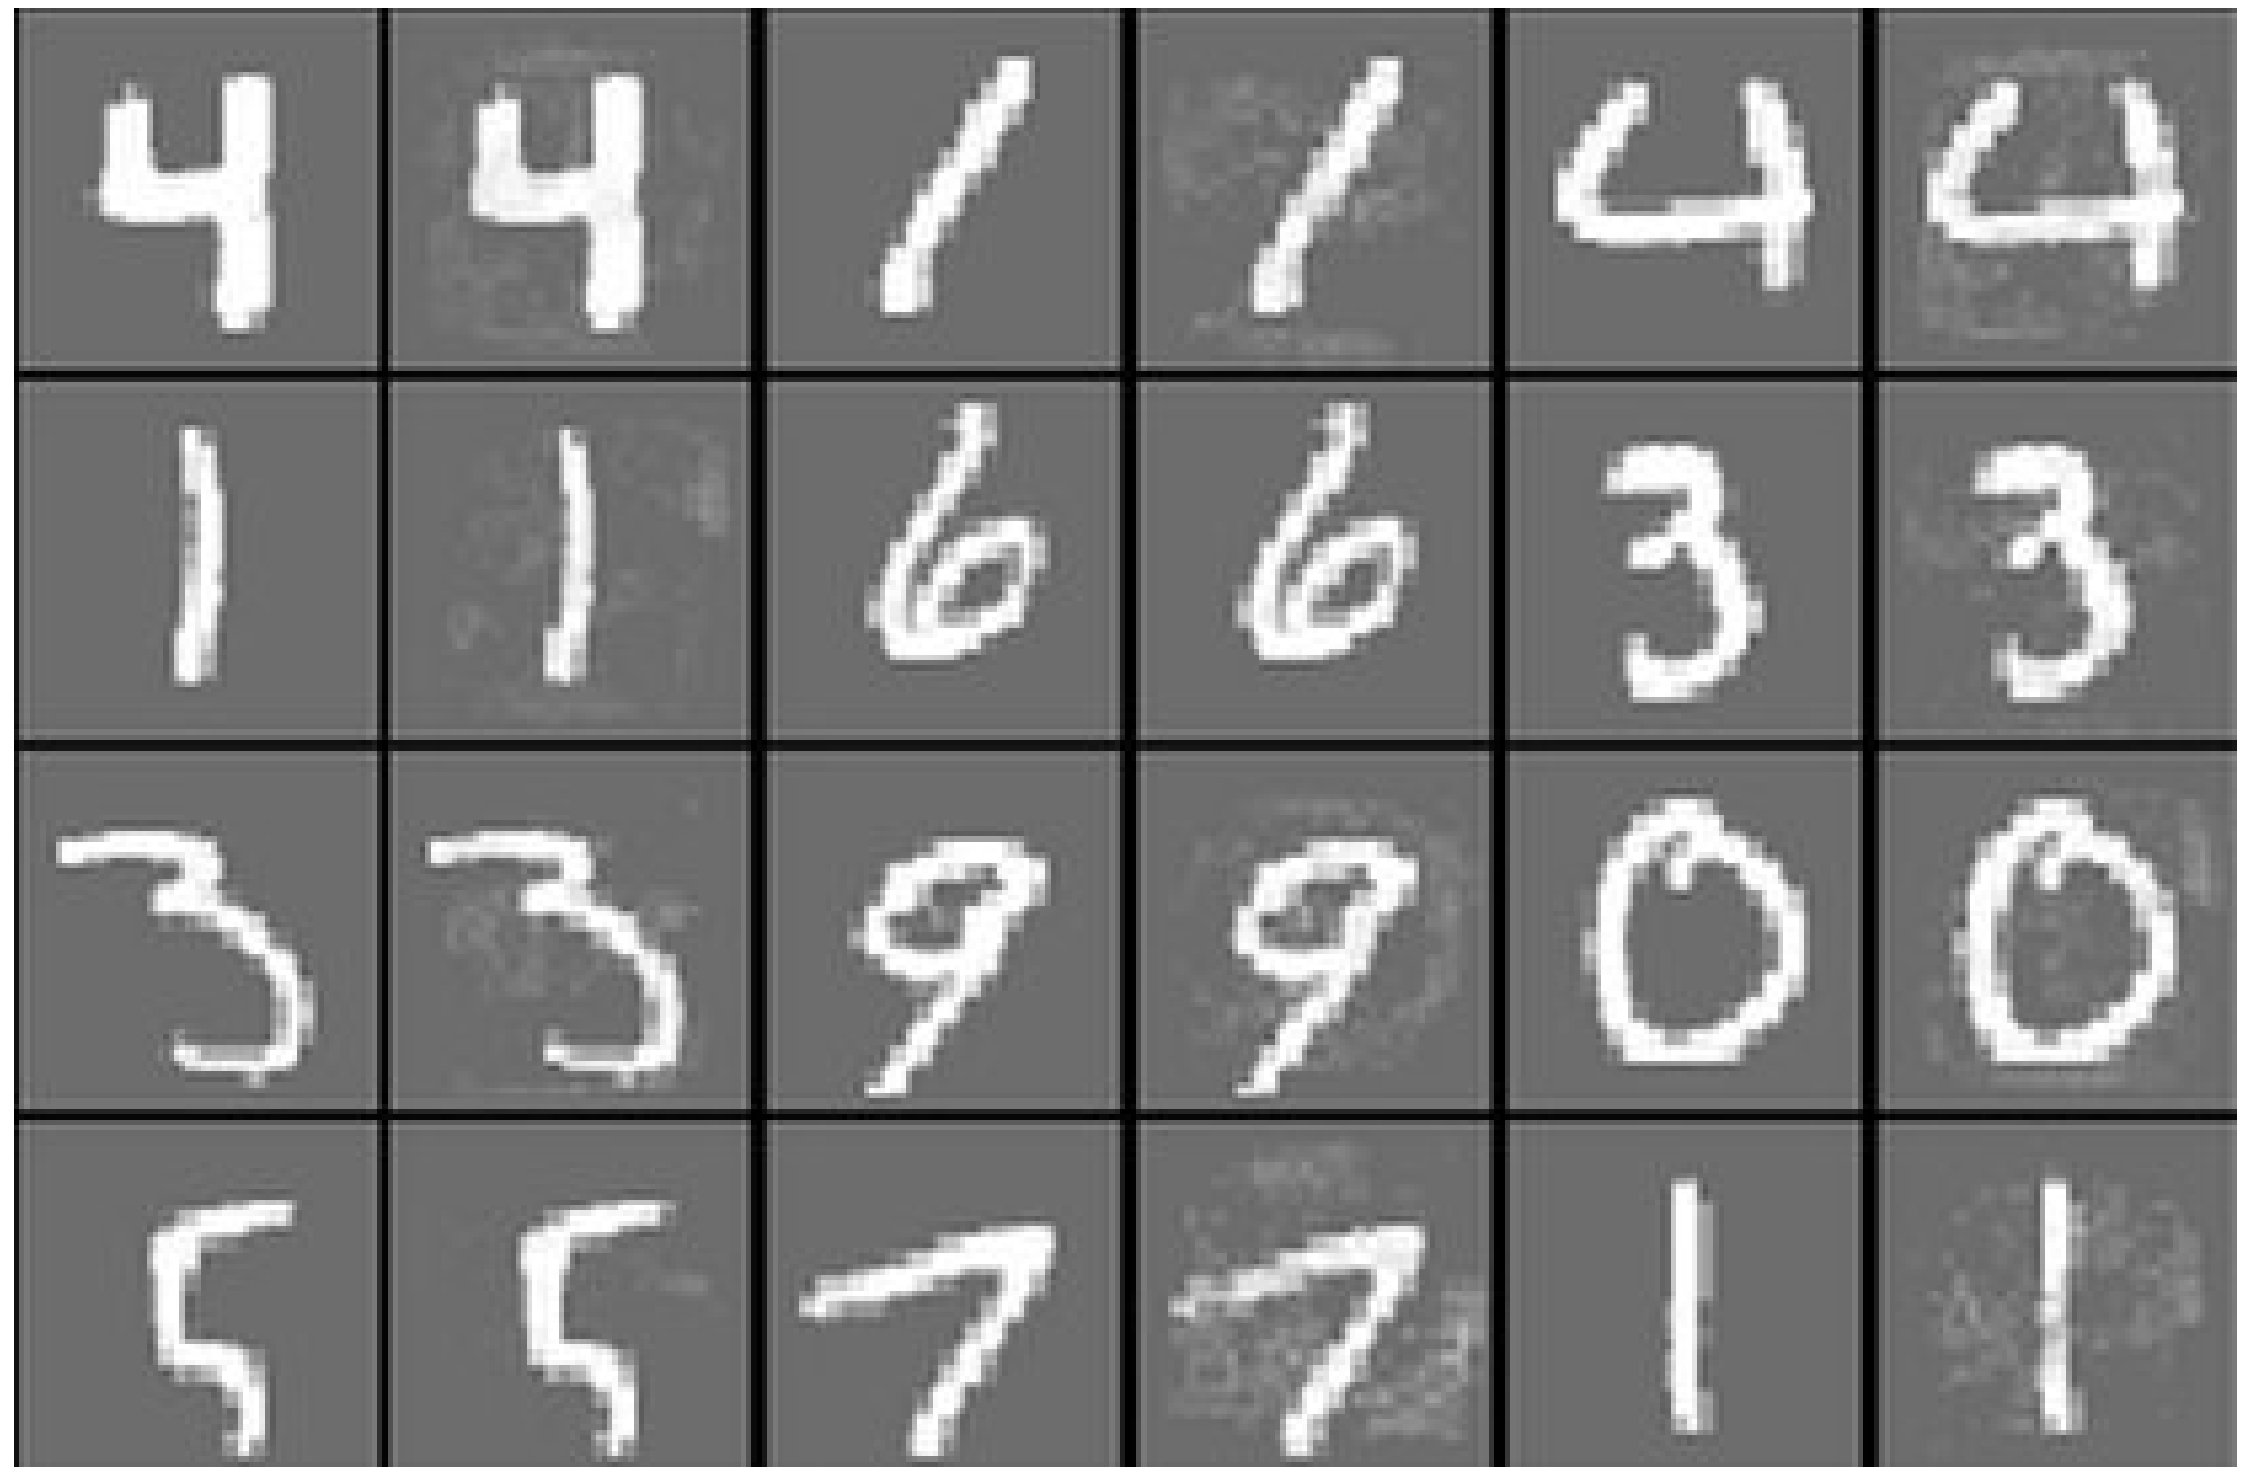
\includegraphics[width = 3in]{Friendly/LaTeX/figures/grid1.png} & 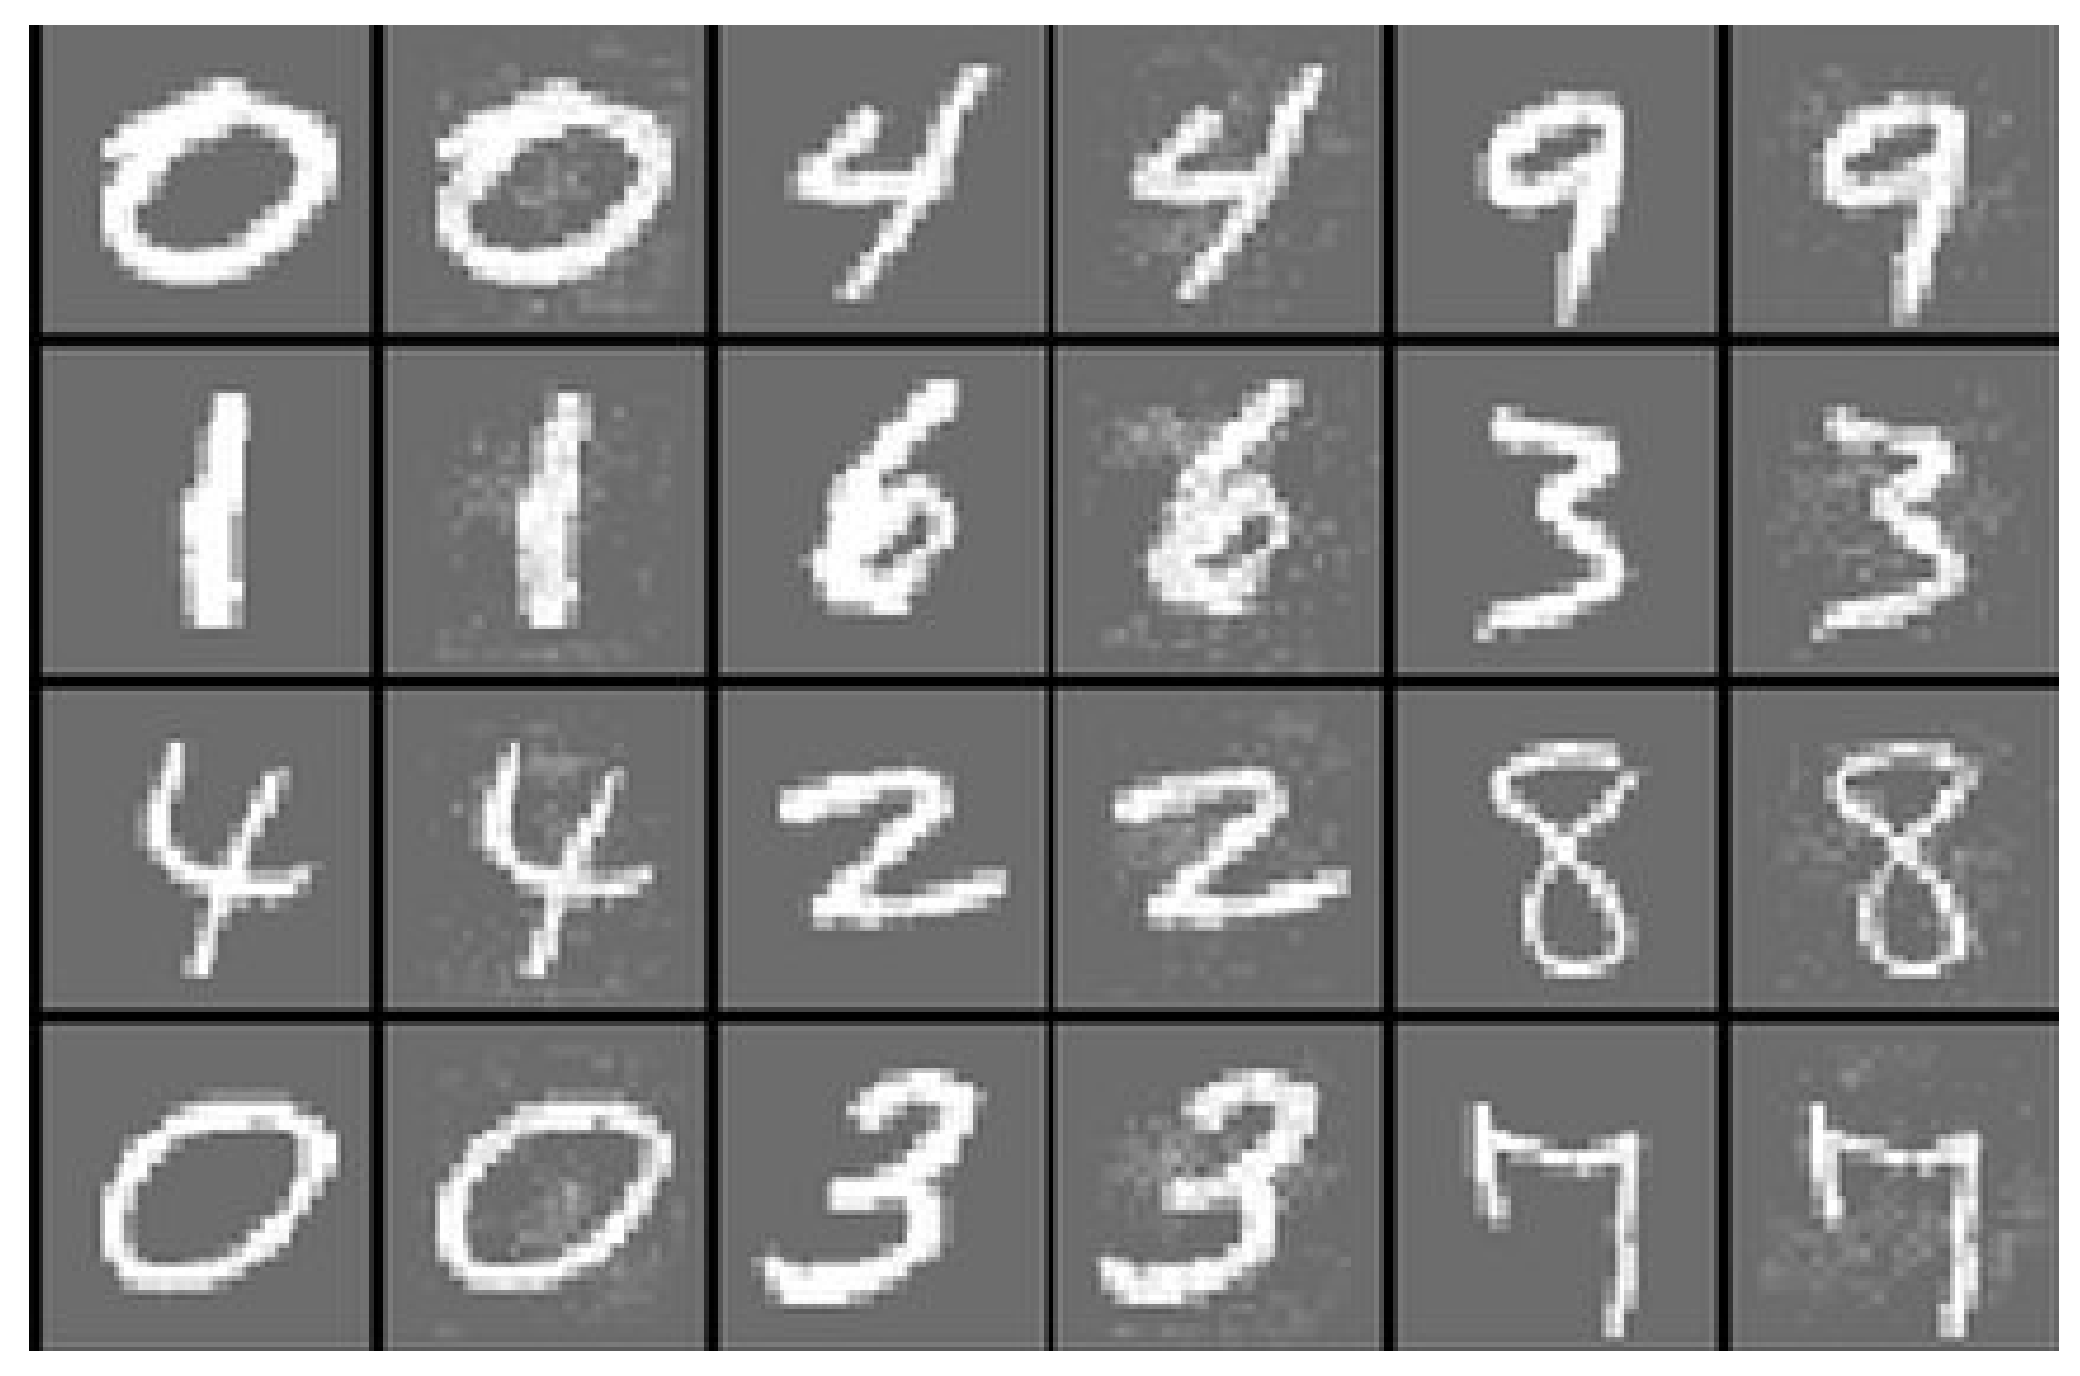
\includegraphics[width = 3in]{Friendly/LaTeX/figures/grid2.png}
        \end{tabular}
    \end{center}
    \caption{Adversarial images taken from ~\cite{szegedy2014intriguing}[figure 7] where the noisy
             images are the adversarial examples. See the figure of that paper for details about
             these images}
    \label{adversarialexamplespictures}
\end{figure}

They also tried to use these adversarial images from one model on the other models. They did this
for each model so that every model in the test was used to generate adversarial examples to be used
on the others. The error rate for the other models was substantially lower; however, the minimum
error rate (of all tests) was still a few times higher than data that had not been disturbed, with a
few error rates well over 70 percent. Further, to eliminate the possibility that this isn't a issue
of using the same dataset, one network was trained on a different subset of the MNIST dataset. For
the two that were trained on the opposing subset, one of them had a different number of neurons than
the other. They say these two differences were tested at once (with the different network) "to study
the cumulative effect of changing the hyperparameters and the training sets at the same
time"\cite{szegedy2014intriguing}[p.\ 8]. The results show that there is roughly an equivalent
contribution, between dataset and model setup, to error rate with sabotaged images at low
magnitudes. However, when they increased the magnitudes of the noise, the shared-training-scenario
dataset caused much more misclassification when compared to having the training sets be the same
when transferring in both directions between the different models.

The final part of the paper tried to analytically quantify the capability an adversarial sample has
to affect the network's ability to classify things correctly. They used an interesting technique of
a establishing series of derivative upper bounds that cascade through the network, resulting in a
cumulative upper bound.